%%%%%%%%%%%%%%%%%%%%%%%%%%%%%%%%%%%%%%%%%%%%%%%%%%%%%%%%%%%%%%%%%%%
%                                                                 %
%                            CHAPTER ONE                          %
%                                                                 %
%%%%%%%%%%%%%%%%%%%%%%%%%%%%%%%%%%%%%%%%%%%%%%%%%%%%%%%%%%%%%%%%%%%

\chapter{INTRODUCTION}

Anyone who has used an iPhone or owned a video game console understands the basics of versioning.
Companies brand sequential devices to indicate improvements in performance or capabilities.
This basic identification method has given rise to a plethora of versioning systems used widely across a landscape of software and data.
They help scientific workflows avoid losing work by managing transitions and changes while in operation \cite{Casati1996}.
They provide necessary documentation which informs the transition to new methods and procedures \cite{Wiil:2000:RDH:338407.338517}.
They provide accountability for the value of a project's dataset when considering an agency's continued funding \cite{Cavanaugh2002}.
As Barkstrom writes in 2003,
\begin{quotation}
	If scientific data production were easy, instruments would
	have stable calibrations and validation activities would discover no need for
	corrections that vary with time. Unfortunately, validation invariably shows that
	instrument calibrations drift and that algorithms need a better physical basis.
\end{quotation} \cite{Barkstrom2003}.

\section{Defining Versions and Versioning}

Using versions in the vernacular has become so pervasive that few documents formally define it.
Barkstrom describes versions as ``homogeneous groupings" used to control, ``production volatility induced by changes in algorithms and coefficients as result of validation and reprocessing," \cite{Barkstrom2003}.
This definition's first implication is that such \textbf{groupings} indicate an expectation that versioning requires multiple objects.
With only one object, all metadata would be homogeneous and groupings would become unnecessary.
Whether in the same or different groups, the relationship between entries informs the grouping necessary to organize the data collection.
Figure \ref{hierarchy} visually displays this concept with each file having a clearly defined grouping at each hierarchical level.
Another implication is that version changes can be determined by studying the difference in provenance between two objects.
Changes in algorithms and coefficients may induce enough volatility into the data that a new grouping becomes necessary.
However, this relies heavily on knowing which provenance changes correspond with resulting volatility.
A new version of a data set can result from modifications to data downstream propagated through a workflow without significant changes to the immediate algorithm or coefficients.
In addition, a deeper investigation would become necessary to quantify the amount of volatility introduced by these changes, and how much is necessary to induce a change at each level of the hierarchy.
Therefore, a version definition cannot rely on provenance alone.

\begin{figure}
	\centering
	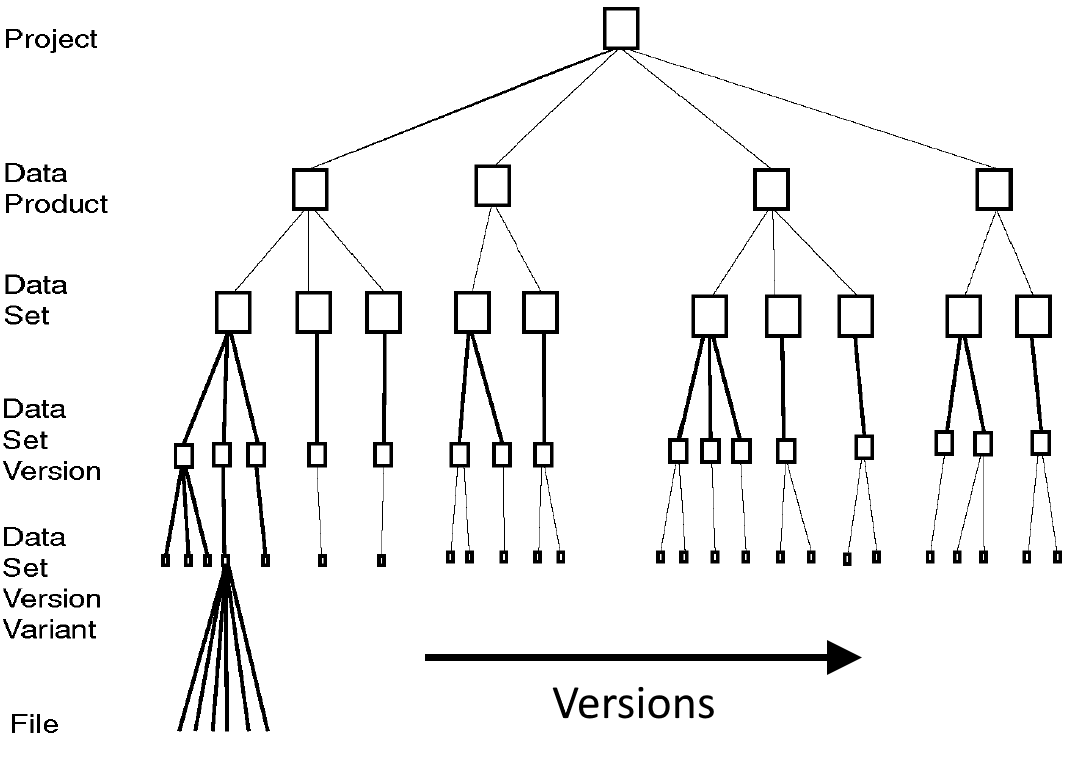
\includegraphics[scale=0.50]{figures/hierarchy.png}
	\caption[Visual representation of grouping hierarchy.]{Visual representation of grouping hierarchy.  From \cite{Barkstrom2003}}
	\label{hierarchy}
\end{figure}

Another definition comes from Tagger in which versions are a, ``semantically meaningful snapshot of a design object," \cite{Tagger2005}.
Unfortunately, he does not further clarify what he means by semantically meaningful.
It is, however, important to note that these snapshots are not of any design object, but the same one.
A similar context connects each snapshot, meaning that they are versions as a result of sharing the same subject and setting.
More specifically, these designs perform the same function in their application.

Combining these conclusions together, a clearer image emerges.
A version is, at its core, a work, but it is not a singular work.
Versions are members of a group which have common, but varying provenance.
However, these members must also perform the same function as others in their group.
This creates specific requirements as to when two objects can be considered versions of each other.

Notice that neither definition includes how to generate versions.
The derivation, PROV Ontology's analog for a version, is defined as, ``a transformation of an entity into another, an update of an entity resulting in a new one, or the construction of a new entity based on a pre-existing entity," \cite{Lebo2013}.
In this view, a version exists because an activity generated it.
However, looking more closely at the forces acting upon the version, they generate an object which becomes a derivation of another as a result of sharing the properties previously mentioned.
The version identifier becomes applied using prior knowledge, not as a result of generation activities.
That is, an activity determines whether an object is a version of another based on the state of that object.
Therefore, versioning is the activity of identifying two objects connected by provenance and exposing the changes relating them, not of generating versions.

\section{Identifiers}

Data managers often impose a sequential ordering in conjunction with logical groupings to form an object's historical lineage \cite{barkstrom2014earth}.
As a result, they often employ version identifiers in the dot-decimal style where a decimal point connects together a series of numbers \cite{Stuckenholz:2005:CEV:1039174.1039197}.
Whenever, a new version is made, it receives an identifier with one of the numbers incremented as seen in Figure \ref{RCSTree}.
Changes to the left-most number often signify a more important change.
Many software applications use the 3-number Major.minor.revision format in labeling software releases.
Numbering the version this way, however, does allow computers and readers to quickly parse the version name and discern that a change has occurred, but not much value exists beyond that \cite{Dijkstra1994}.
Most importantly, it groups together changes from the lower spectrum of minor or major change with those in the upper, more impactful, changes.
It is, therefore, difficult to obtain a clear characterization of a version change without a longer series of numbers.
This method of identification also has issues since small changes in the current data set may have larger implications for data farther down the workflow, which is not communicated by the identifier.
In addition, version numbers capture the overall change of a data set, but users may not interact with collections that way.
Data on a hurricane sometimes occupy only a small portion of a data set, and the files may not even be adjacent in the collection \cite{Barkstrom_digitallibrary}.
There is also little standardization or formal requirements in naming methods.
Ubuntu utilizes a dot-decimal version labeling scheme where the two number identifier corresponds to the year-month values of the release \cite{Ubuntu}.
Fischer, et al., demonstrate the importance of having a regular standardized version identification system, as it provides a mechanism to track errors being addressed \cite{Fischer2003}.
The ability to link bug reports and versions thus gives producers and customers metrics to understand how developers fix errors and how long it will take.
A common method used to address the distinction between versions is a human-readable change log, further discussed in Section \ref{sec:changelog}.


\begin{figure}
	\centering
	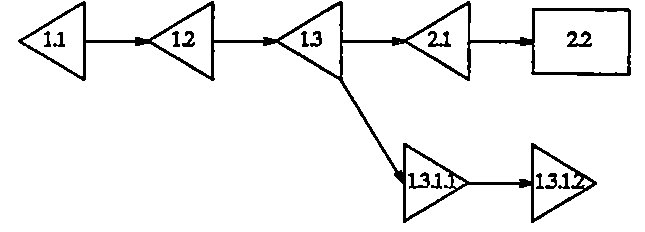
\includegraphics[scale=0.75]{figures/RCSCommitTree.png}
	\caption[Commit history of an object in RCS with changes in the main line stored as back deltas and side branches stored as forward deltas.]{Commit history of an object in RCS with changes in the main line stored as back deltas and side branches stored as forward deltas.  Figure 5 in \cite{tichy1985rcs}}
	\label{RCSTree}
\end{figure}

In many ways, versioned objects resemble multi-edition books or documents.
Digital librarians have faced many challenges when searching for an identifier due to evolving web technologies.
Early citations referred to on-line documents using stagnant Uniform Resource Locators (URL), but this frequently lead to a condition known as link rot where moving the document would invalidate the URL \cite{Lyons2005}.
Locators required a system to manage changes of old identifiers to new locations when people attempted to utilize references from print.
This eventually led to the development of Persistent URLs (PURL), which also suffered from link rot, and this eventually led to the distributed Digital Object Identifier (DOI) system used to track documents today \cite{Duerr2011}.
The PURL used a centralized system that would translate dead links and redirect to a document's latest location.
However, the system would still need to be manually updated, meaning links would rot if a document was lost or overlooked.
DOIs rely on a network of managing agencies to collect and host submitted documents.
In the specialized Handle system, the network has member agencies internally assign an unique name and concatenate it to the end of their host name.
In Figure \ref{table:Duerr}, DOIs represent the most suitable identifier used for citation in scholarly literature \cite{Duerr2011}.
The DOI network provides a robust system to track documents, but when tracking data, it faces difficulty following the rate of change with more volatile data sets.
Under current definitions, distribution organizations assign different DOIs to separate editions of a document.
Documents often do not need new identifiers since they change very rarely as a result of the publication process.
However, the data set production and distribution cycle moves more quickly and reacts more sensitively to small content changes, including when data collection continues on after initial publication.
This behavior becomes entirely too slow as data providers begin allowing users to dynamically generate data products from existing data according to their needs \cite{Barkstrom2003a}.
Some agencies have begun assigning versioned DOIs, but this has not become common practice.
Other groups do not assign a new DOI, but reference to the latest release of the document or object \cite{Ands2017}.
As data sets continue to grow in size, it may become impractical to look towards data as the driving source for identifiers, as Proell and Rauber suggest that database queries may provide a more scalable means of citing datasets \cite{proellBigData}.

\begin{figure}
	\centering
	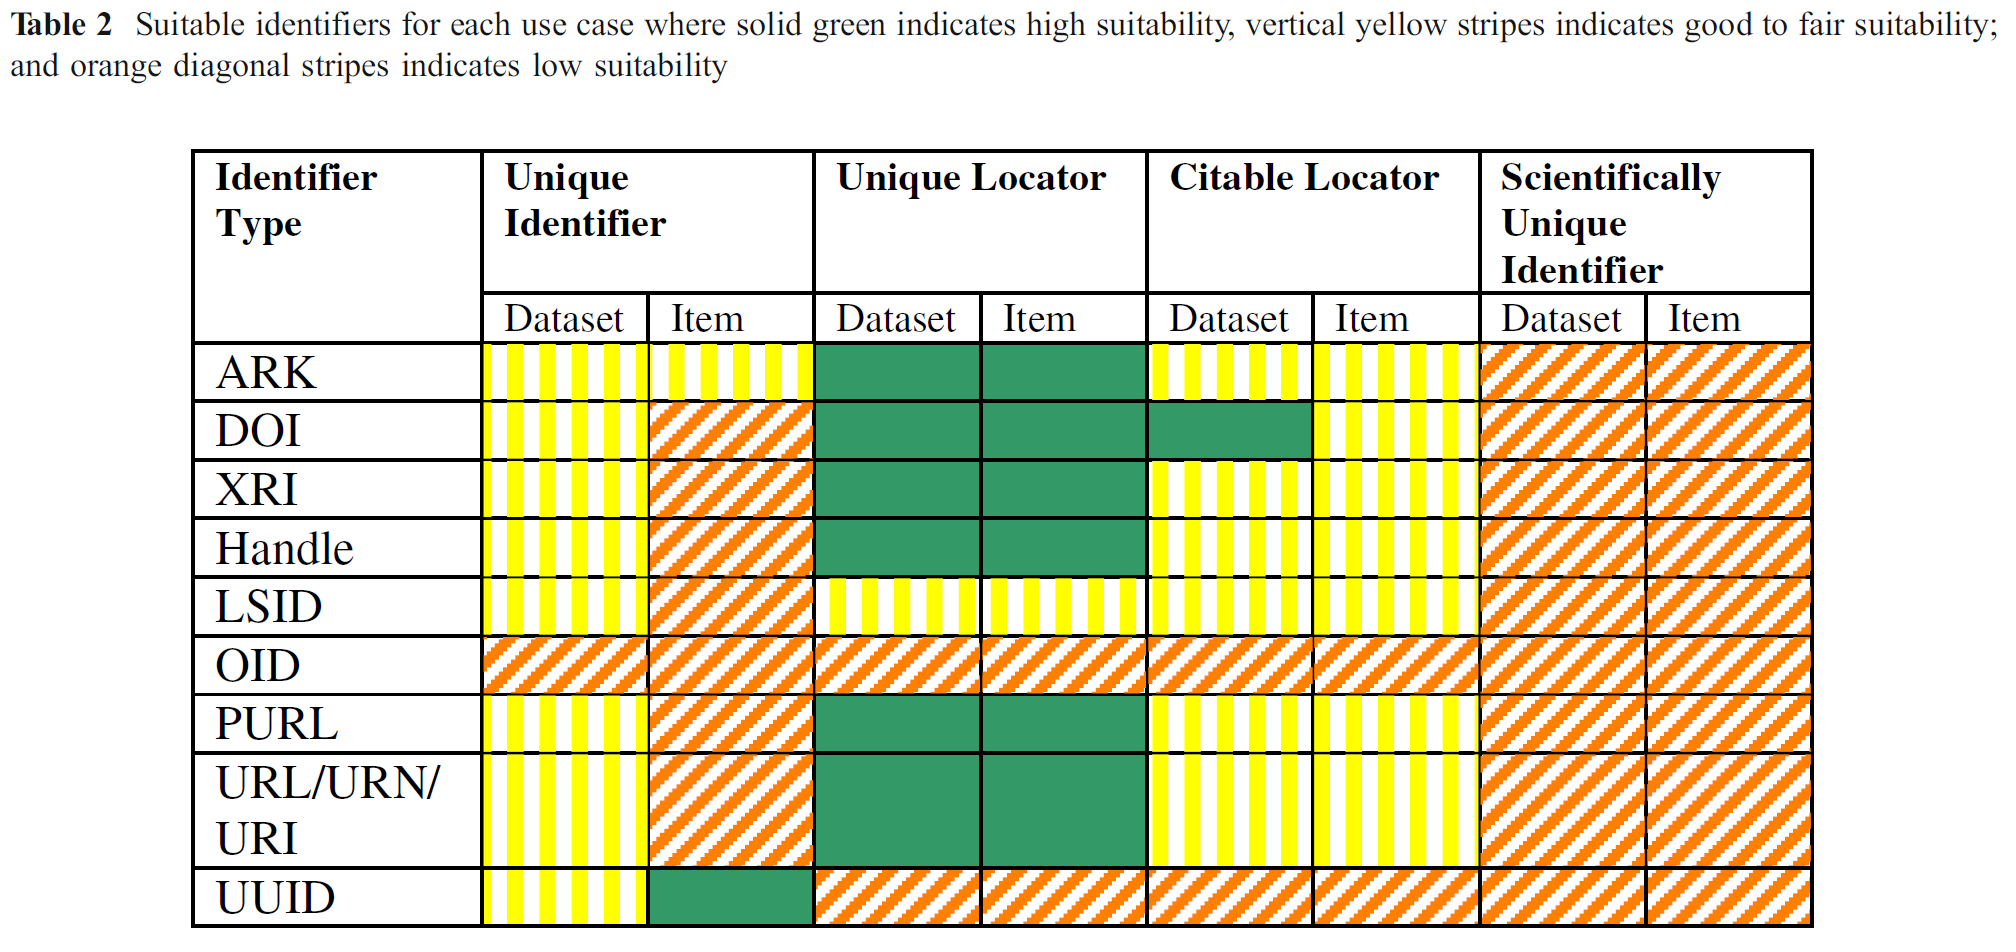
\includegraphics[scale=0.30]{figures/DigitalIdentifierTable.png}
	\caption[Table of predominant identifiers used in science.]{Table of predominant identifiers used in science.  From Duerr, et al. \cite{Duerr2011}}
	\label{table:Duerr}
\end{figure}

The discourse on DOIs highlights the importance of understanding the limitations of particular identifier schemes.
With respect to Figure \ref{table:Duerr}, no identification scheme fits the description of a scientific identifier.
Duerr, et al., define a use case to make the argument that scientifically unique identifiers are necessary, ``to be able to tell that two data instances contain the same information even if the formats are different" \cite{Duerr2011}.
A possibility to consider is that identifiers may require incorporation into a data model to discern between scientific differences.
An identifier works well in revealing the characteristics of an individual object, but it should not be expected to explain its relationship with other objects.
A data model provides better insight into the different roles objects play in a relationship.
Further discussion on versioning models will be found in Section \ref{sec:models}.
This proves increasingly important as the ability to propagate relevant data change across autonomous systems then assures valid quality in interactions between domains \cite{Systems02champagne:data}.

Using identifiers to convey extended versioning information becomes more difficult with the adoption of distributed version managers like GIT \cite{cederqvist2002version}.
Each participant in the federated repository is the master of their personal copy of the code.
Upon completion of their distribution's part, they may request that it be pulled into another participant's distribution.
While each developer's individual repository can follow a linear identifier scheme, this would not work as the overall project bounces around different primary repositories with mismatching sequential identifiers.
The dot-decimal identifier scheme could be made to work in such an environment by severely limiting the distributed manager's utilized features.
Figure \ref{fig:federated} illustrates a workflow which utilizes distributed repositories to manage very active public software projects.
Each lieutenant developer manages a section of the overall code, and they dampen the number of requests made to the dictator by collecting changes and submitting them over longer intervals.
As a result, relying on identifiers to convey and contain versioning information limits the evolution of new and valuable methods of processing change in digital objects.

\begin{figure}
	\centering
	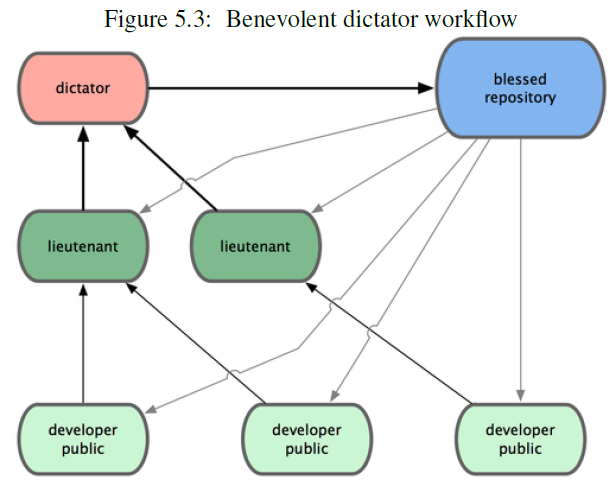
\includegraphics[scale=0.85]{figures/federatedGit.png}
	\caption[A distributed workflow to control for volatile versioning behavior.]{A distributed workflow to control for volatile versioning behavior.  From  \cite{cederqvist2002version}.}
	\label{fig:federated}
\end{figure}

\section{Change Logs} \label{sec:changelog}

Change logs, artifacts resulting from the versioning process, play a major role filling in gaps between versions.
They document changes and explain, in human language, the motivations behind these modifications \cite{uel1037}.
Since identifiers denote that a change has occurred, the logs provide details on how the changes modify an object's attributes.
They demonstrate a need and utility in understanding the deeper content of change beyond knowing that an object did transform.
While some data sets will provide a change log, software projects have normalized their use in version release documentation.
As a result, these projects provide a basis for understanding the value these logs can supply data sets with multiple versions.
The change log's common drawback is the limitation to only human readable text.
Wider adoption among data sets may be possible by making these texts machine computable.

Open source projects use change logs more consistently than data projects, which usually sport only use documentation.
Logs play an important communication role in these projects since developers can contribute without having been part of the original development team.
They allow developers to link bugs and errors with their corrections in new versions of the code \cite{Chen:2004:OCL:990374.990391}.
This gives insight into motivations behind particular design decisions.
It also provides feedback to the user community that corrections have been addressed, in addition to ensuring that improvements drive modifications to the code base.
An identifier cannot communicate these qualities while remaining succinct.
Some research has been done to determine the health of a development project based on the number and length of change logs released over time \cite{German03automatingthe}.
This becomes particularly significant as data freshness plays a growing role in successful system function \cite{Bouzeghoub:2004:FAD:1012453.1012464}.
However, little work has been done to make change logs machine-computable, as many of these documents remain in human-readable text only.
Research done involving change log content must manually link entries with computable meta-data such as the introduction of new features with the emergence of new bugs \cite{6132954}.
While machines may still be significantly removed from the ability to comprehend the impact of changes made to a data set or software code, they are currently opaquely blocked from consuming any of the content within logs more than understanding they contain text.
The transition between different versions of large datasets is then left largely up to the human user's ability to understand and process the modifications mentioned within the change log.

\subsection{Structured Data}

The Resource Description Framework in Attributes (RDFa) framework encodes linked data vocabularies into HTML documents, and provides an opportunity to make change logs machine interpretable. \cite{Adida2015}.
Linked data technologies utilize web ontologies to standardize terms and semantics across domain applications.
Automated agents can reason over a graph formed by linking these terms.
Encoding HTML documents with linked data better unlocks the content stored within.
\begin{figure}
	\centering
	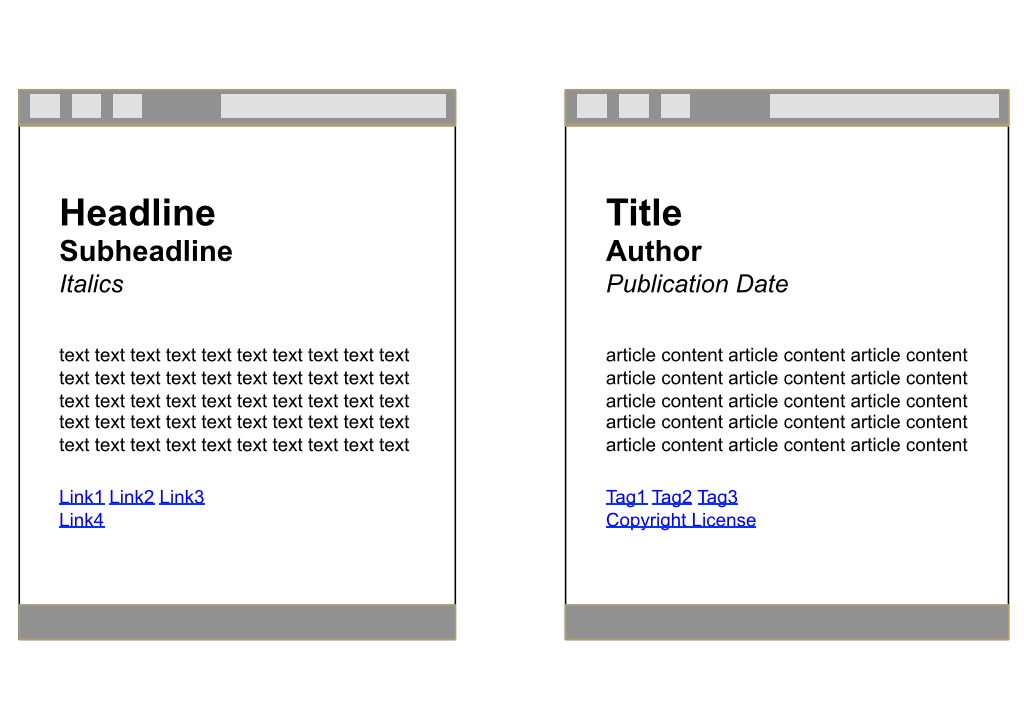
\includegraphics[scale=0.40]{figures/RDFaSemantics.png}
	\caption[Illustration of the difference in what autonomous systems see when crawling a web page and what humans see when reading the same material.]{Illustration of the difference in what autonomous systems see when crawling a web page and what humans see when reading the same material. Figure 1 from \cite{Herman2015}}
	\label{RDFa}
\end{figure}Figure \ref{RDFa} illustrates the semantic difference between what web crawlers and what humans see when they consume web pages.
People intuitively understand that certain strings represent meaningful information based on location and style.
RDFa seeks to encode that understanding natively for effective machine consumption.
Extending this approach into publishing change logs, will allow linked data to capture the metaphorical meat of change content.

The implementation requires changing publishing practices from plain-text documents to something structured-data compatible such as HTML.
The change also has the added benefit of making the logs available on-line, and thus, more openly accessible to data users through the utilization of web based search engines.
Large companies such as Google have already begun equipping their web crawlers to consume structured data such as RDFa from web pages.
RDFa has already had significant success in adoption across a variety of web publication platforms and eases the search for their content \cite{Bizer2013}.
However, the design of RDFa focuses on describing the web page's content through markup \cite{Herman2015}.
The underlying or resulting versioning data model may not conform with the format of content presented in the change log.
This would lead to a poorly structured graph or missing content, undermining the value gained by encoding linked data into the change log.
As a result, another method using JavaScript Object Notation for Linked Data (JSON-LD) was pursued since its purpose is to store data separate from visible content.

The JSON data format allows web pages to store data for JavaScript applications within the document.
It utilizes a simple and robust syntax to accommodate a wide variety of content.
JSON-LD extends the original specification by defining rules which allow entries to resolve as web vocabularies, giving them a meaningful context \cite{JSONLD}.
Because it stores data separate from visible content, JSON-LD does not need to adhere with the constraints of visible content.
However, every linked data triple must be explicitly defined, meaning that resulting documents may likely be much larger than their RDFa counterparts.

\section{Modeling} \label{sec:models}

Initial research in version modeling occurred with databases, studying ways to track and migrate schema changes.
Capturing periodic snapshots or copies becomes unfeasible with increasingly large centralized database systems.
This gave rise to the first temporal databases where schemas included time and dated transactions modifying the schema \cite{roddick1996model}.
This provides the database a method to transactionally rollback the environment to recreate a search.
As databases grew more complex, the intricate relationships between objects made rollbacks more difficult.
This results from the need to manage the time instances of realization, storage, and validity.
The datum becomes realized at collection, then stored upon entry into the database, and finally valid until the present or new data replaces it.
Klahold, et al., introduced using abstract versioning environments to separate the temporal features and organize them into related groupings \cite{Klahold:1986:GMV:645913.671314}.
As publications more often include citations to data, researchers adjust to enormous modern databases with new methods changing queries rather than transforming schemas \cite{Proell2013} \cite{DBLP:conf/data/2013}.
This method, however, relies on an abstract model capturing data changes to inform query modifications.

Data models allow the capture of complicated relationships between data objects within a system without needing to physically look over sizable datasets.
The Proof Markup Language, one of the first semantic models to capture provenance information, expressed these relationships using inference reasoning through traceable graphs \cite{daSilva2006381}.
Many data models include versioning concepts in their specifications, but they are often provenance models which describe the sequence of events that lead to the construction of an object \cite{dai2014provenance}.
However, as discussed previously, versioning seeks to expose relationships between objects which may not describe how to construct either one.
The Health Care and Life Sciences (HCLS) Interest Group recently released a model which may provide a solution when used in conjunction with other identifiers \cite{Dummontier2016}.
Their model, shown in Figure \ref{HCLSModel}, separates the concept of a dataset into three groupings.
The highest level summarizes the data as an abstract work, perhaps better described as a topic or title.
This data topic can have multiple versions as it changes over time.
The version can then be instantiated into various distributions with different formats.
Compare this to the diagram in Figure \ref{hierarchy} which features more tiers.
In this case, the basis for diverging groups is changes in identifier and physical formating of that version.
This model also demonstrates how it can better communicate scientific similarity than an identifier.
The model logically links together, under a single version, representations of that data adjusting for physical perturbations.

\begin{figure}%[b]
	\centering
	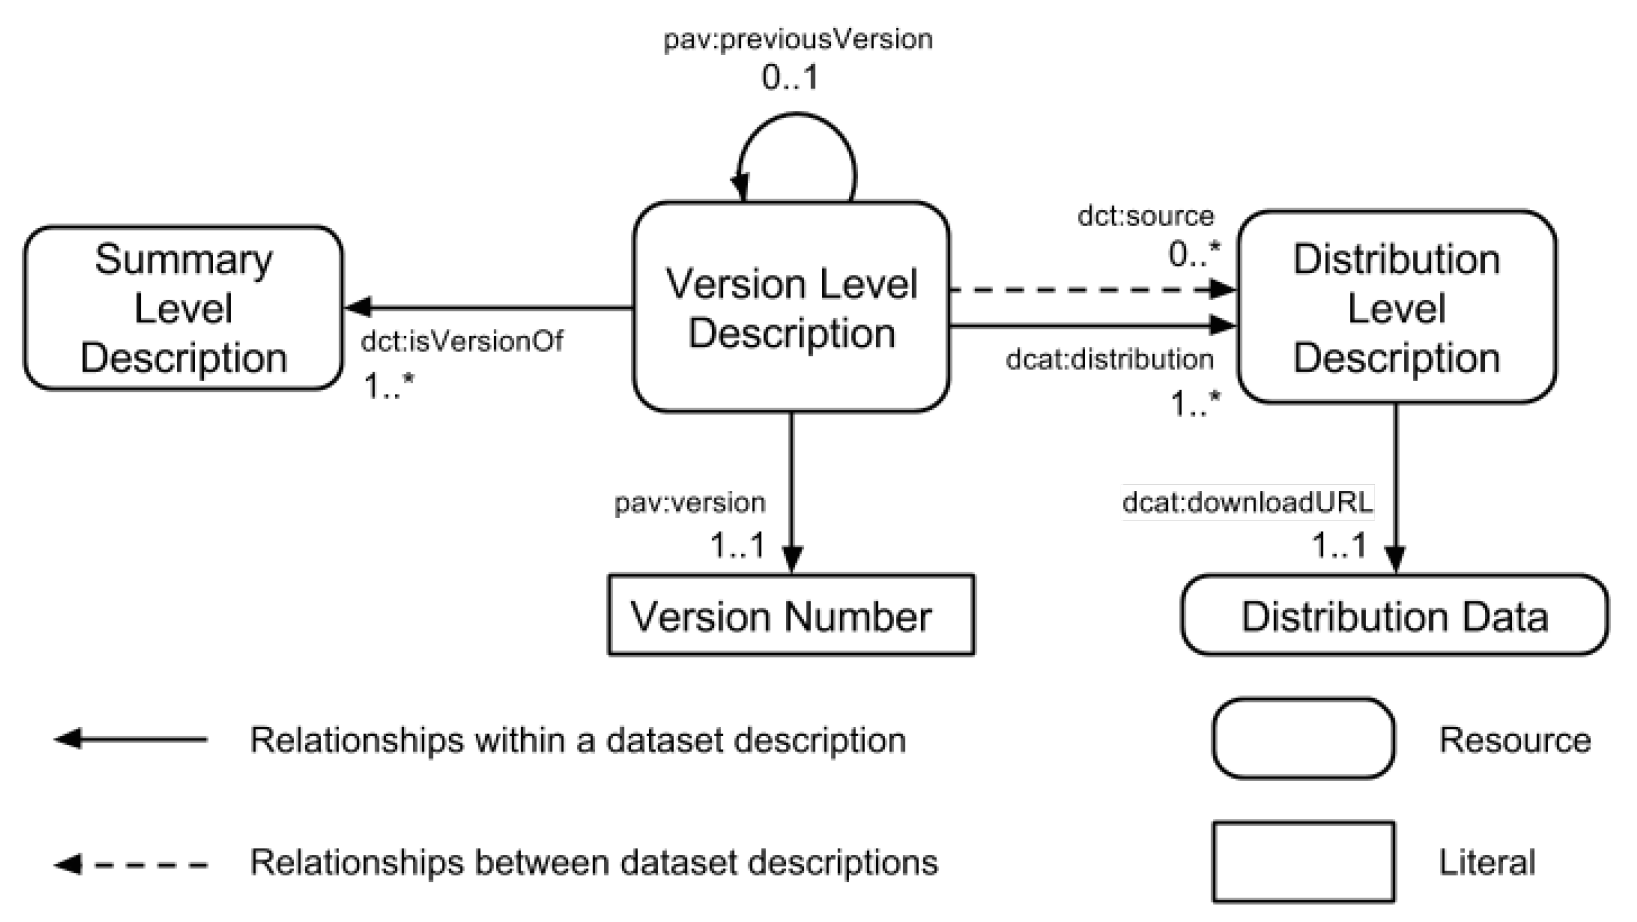
\includegraphics[scale=0.35]{figures/HCLSModel.png}
	\caption[Data model from the Health Care and Life Sciences Interest Group separating data into three levels: works, versions, and instances.]{Data model from the Health Care and Life Sciences Interest Group separating data into three levels: works, versions, and instances.  From Dummontier, et al. \cite{Dummontier2016}}
	\label{HCLSModel}
\end{figure}

The HCLS data model captures version information using the Provenance, Authoring, and Versioning (PAV) ontology \cite{Ciccarese2013}.
As explained in their document, PAV addresses versioning as a result of disagreements with other ontologies' definitions such as PROV.
They enumerate specific situations relating to health care data requiring broader conceptual coverage.
As a result, their model provides basic properties to identify a previous version and its corresponding identifier.
They do not provide methods to identify motivations or discuss the role attribute differences effect changing versions.
The existence and widespread adoption of change logs demonstrates the importance of this information in understanding modifications between versions.
However, PAV does adopt a state-based perspective regarding versioning since it only seeks to identify a previous version without attributing a responsible activity.

The PROV data model is a World Wide Web Consortium (W3C) recommendation which defines linked data properties to capture data provenance \cite{Gil2013}.
PROV has played a significant contribution in maintaining the quality and reproducibility of datasets and reporting in the National Climate Assessment (NCA) \cite{Ma2014191}.
This implication signifies that there is an increased likelihood of adoption through other scientific fields as a result of this reporting.
The Global Change Information System, which houses the data used to generate the NCA, uses PROV to meticulously track the generation of its artifacts and results as they are used in the report \cite{Tilmes2012}.
This means that not only does the data have a traceable lineage to verify quality, but the content of documents can have the same verifiability \cite{Ma2014}.
While a subtree of terms deal with versions, the ontology takes an activity based view of data.
This makes sense since it seeks to explain what activities led to the creation of an object.
This focus on activities results in a very shallow definition of methods to capture entity-to-entity relationships within the model.

\begin{figure}
	\centering
	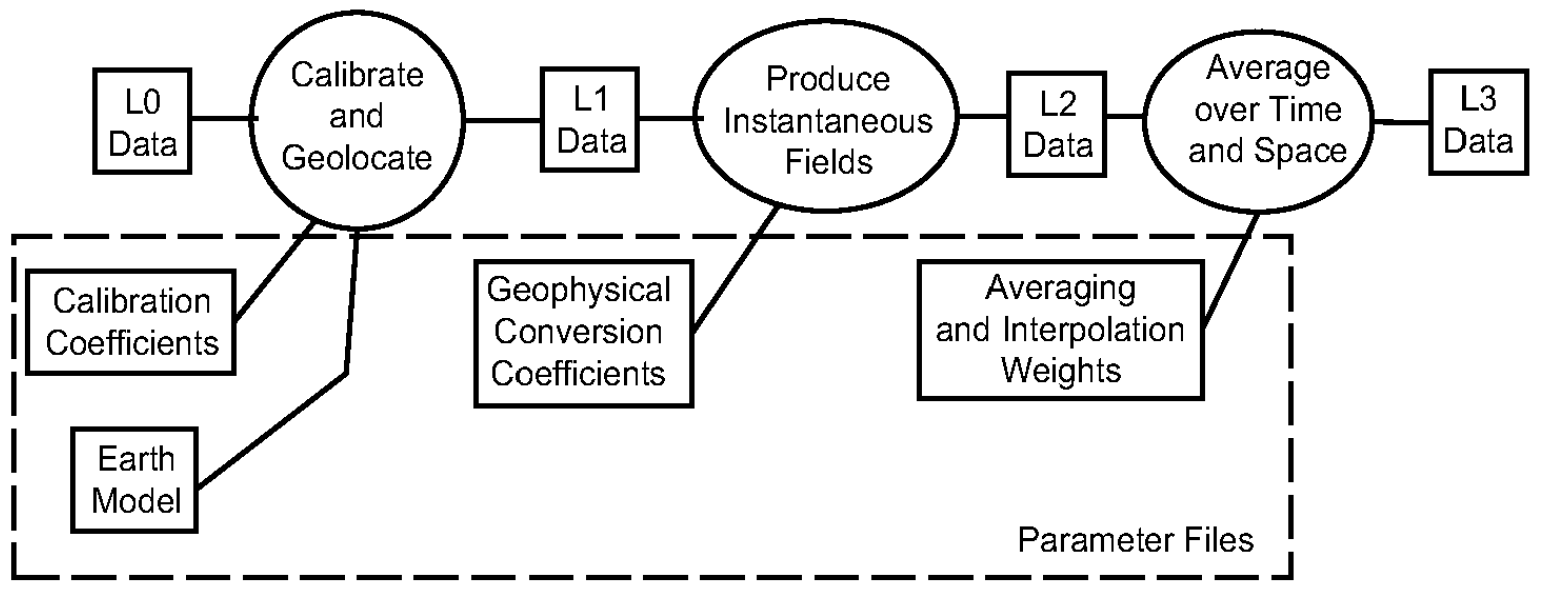
\includegraphics[scale=0.35]{figures/NASALevels.png}
	\caption[NASA organizes its data into three levels depending on the amount of aggregation and the distance the data is removed from the original sensor measurements.]{NASA organizes its data into three levels depending on the amount of aggregation and the distance the data is removed from the original sensor measurements. Figure 1 from \cite{Barkstrom2003}}
	\label{NASALevels}
\end{figure}

In his discourse on version management, Barkstrom introduces NASA's workflow model as seen in Figure \ref{NASALevels}.
It describes the formal stages of processing to turn a raw remote sensing signal from satellite instruments into global aggregate summaries \cite{Barkstrom2003}.
Understanding this model reveals that changes to either the algorithms or parameter files will force a change in the resulting data.
This explains the new result's provenance, but it would not capture the differences between these objects.
The key to understanding version modeling lies in recognizing provenance and versioning are intimately entwined, but seek to explain different properties about data objects.

Klein and Fensel determined versioning systems needed to capture compatibility as a major characteristic while performing a study of different ontology versioning methods \cite{Klein01ontologyversioning}.
There are two types of compatibility, `forwards', which explains how to modify old data to work with new content, and `backwards', which allows new data to interact with old data.
Knowing one type of compatibility does not always entail the means of deriving the other.
Having full forwards and backwards compatibility allows interoperability between a variety of applications which may use different versions of the same ontology.
However, it often depends on the application as to whether full compatibility is necessary.
Once concern which is very rarely discussed is the compatibility of files and objects which do not change at all.
Take, for example, some biological ontologies, which must update terms and definitions to better capture the field \cite{Ochs:2015:SVS:2826733.2826866}.
They mention very little on how to migrate terms which do not change, but these can contribute to a majority of copied content and pose significant scaling issues.

\section{Data Versioning Operations}

Versioning systems come in a variety of different forms as a result of the assorted applications they must manage.
Experimental biology data require tracking as they pass through a scientific workflow \cite{Tagger2005}.
Libraries curate multiple editions of the same work, sometimes with significant revisions \cite{Wiil:2000:RDH:338407.338517}.
What such activities demonstrate is the wide range of settings and expectations under which versioning systems operate.
While this work cannot hope to explore all these applications, every system studied shares three common functions: addition, deletion, and modification.
These three operations plausibly form the core set of relationships when versioning.

Literature surveys often expect versioning systems to interact with data uniformly because they are asked to perform the same functions \cite{Tagger2005}.
However, different data sets may utilize each of the three core operations at different rates \cite{rohtua}.
This helps to characterize the data set in ways such as a growing set with many additions, a stable collection featuring occasional corrections, or a wildly volatile data set consisting of often deleted and replaced data files.
Understanding these would give insight into the maturity and health of a dataset, but most major provenance ontologies do not heavily feature these relationships.
Versioning information, of course, does not give insight into the origins of an object, and therefore, would not be expected to play a major role in provenance documentation.

While data addition and modification remain fairly uncontroversial, there is a mild division between practical and theoretical approaches to data deletion \cite{Flouris04clotho:transparent}.
A removed object provides evidence of an erroneous activity's results or intermediary steps leading to a final product.
As a result, version management should maintain and track invalidated data.
The software versioning manager GIT uses a method of compressing older data to conserve space without deleting the data \cite{Chacon:2009:PG:1618548}.
Available storage space places pragmatic constraints on the number of projects which can adopt snapshotting practices.
In applications which cannot recover erroneous data nor use it as documentation artifacts, like corrupted surveillance images.
Some high energy physics experiments cannot re-collect observational data due to cost, and as a result, they cannot replace or re-process poor quality data \cite{Cavanaugh2002}.
While the distinction between `deletion' and `invalidations' remains largely semantic, the terms' use in this document reflects an understanding of the different constraints and requirements placed on versioning systems.
As a result, invalidation is adopted as a broad, general term to also encompass data deletions.

A handful of other operations exist among version managers, but they do not prove ubiquitous across most applications.
Software versioning tools like RCS commonly feature branching and merging functions to create a versioning line separate from the stable master branch \cite{tichy1985rcs}.
This mostly provides an organizational role in development by allowing developers to experiment without contaminating a stable software release.
Figure \ref{GITTree} models this, showing versions C3 and C5 in branch iss53 before being merged back into the production line as C6.
It allows for more orderly management of versions, but does not conduct versioning itself.
Other activities provide functional operations such as locking and unlocking files from edits to prevent race conditions in branch mergers.
It does not introduce any new relationships but allows the tool to operate more smoothly.
Clotho, a versioning application managing versions at the block level, coordinates constrained spaces using intermittent compact and un-compact methods when retrieving or storing old objects \cite{Flouris04clotho:transparent}.
Likewise, many version control tools include functions to display the versioning tree, but this is also an ease-of-use function \cite{Dijkstra1994}.

\begin{figure}
	\centering
	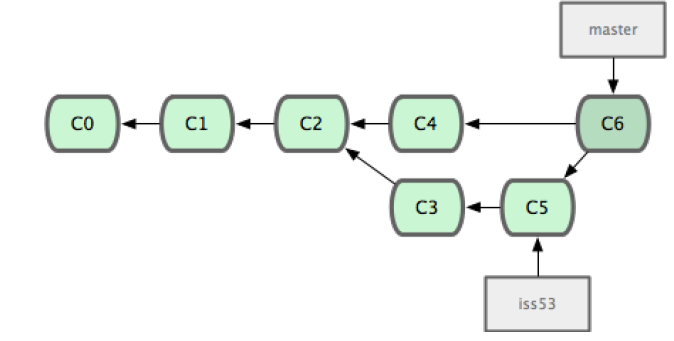
\includegraphics[scale=0.75]{figures/GITCommitTree.png}
	\caption[Example of a commit history with branching stored in GIT.]{Example of a commit history with branching stored in GIT.  Figure 3.17 from \cite{Chacon:2009:PG:1618548}}
	\label{GITTree}
\end{figure}

\subsection{Types of Change}

Barkstrom uses the ability to scientifically distinguish between two data sets as a criteria for major divisions among groupings \cite{Barkstrom2003}.
At lower levels, he notes that science teams can no longer discern scientific differences between data sets.
Instead, they observe that changes to format and structure contribute significant alterations without changing any values withing the data.
As a result, these technical changes form a second boundary to meaningfully separate minor version groupings.
Finally, the explicit values may need occasional revisions to correct lexical errors such as spelling or formatting.
These terms were chosen carefully as they reflect the three value dot-decimal identifier system.
However, data producers will often use qualitative measures to determine the type of change occurring between versions.
Versioning system users wish to achieve insight into the type of change that occurs between versions, and quantitative analysis on versioning operations will provide quantifiable evidence in characterizing the impact of a change.

The exact category that a particular change falls into can be controversial.
The decision to provide concentration units from parts per million to milligrams per milliliter poses a Technical change for a data producer.
However, for a data consumer, the alteration may be viewed as a Scientific change as it invalidates the methods they had previously used.
This conflict in view illustrates the data consumer-producer dynamic.
In general, data producers control the versioning methods, but data consumers determine the classification of a data change.
Producers tend to use versioning systems to ensure data quality of service through audits and recovery tools \cite{Cavanaugh2002}.
Meanwhile, a consumer will analyze the historical changes and determine the impact this may have on their data use.
As a result, this means that data versioning systems must communicate a dynamic view of the changes in a system contextualized by the user of that data.

Version managers often disagree at the point many technical changes sufficiently modifies a data set that it comprises a scientific change.
As determining changes in science requires expert understanding over a domain, different measures should be explored to address the distinction.
This document's approach studies add, invalidate, and modify counts to quantify the impact of changes and how they relate to the producer's observations.
As previously mentioned, different systems utilize the operations at varying rates so absolute cutoffs will be unlikely in comparison to relative results.

\section{Thesis Statement}

Large data collection endeavors necessitate the development and deployment of versioning systems to manage change propagating through their data.
Advancing beyond identifier comparisons and delving into capturing substantive change can significantly improve the ability to standardize version communications and transition.
A model is developed to provide a foundation in regularizing the versioning process and communicating that in a machine-computable manner using linked data.
For this purpose, we compare two methods in micro-data with JSON-LD expected to provide better performance.
These relations cannot be communicated by current provenance models' semantics.
Furthermore, the model provides a quantitative basis for determining meaningful version identifiers following a numerical system which has previously only been performed using qualitative methods.
Through sub-classing concepts within this versioning model, versions can provide detailed comparisons to support experimental designs and decisions.


%%% Local Variables:
%%% mode: latex
%%% TeX-master: t
%%% End:
